\chapter{Scattering}
\section{Classical Scattering}
\subsection{Motivation}
We can also define the size/radius of the proton is through its rate of interacting with 	itself or other particles.
This is done by us determining the cross-sectional area. The larger this area is, the more likely it is that you will interact with it. The smaller the area, the less likely to interact.
This motivates a connection between proton size and scattering probability. In particle physics, a collision or interaction rate is expressed in effective cross-sectional area, typically just called cross section.
As an	“area,” we can measure scattering cross sections as the square of some relevant 	length scale.

\subsection{The problem}
Consider a particle incident on some scattering center. It comes in with an energy \textrm{\textit{\textbf{E}}} and an impact parameter \textrm{\textit{\textbf{b}}}, and it emerges at some scattering angle \textrm{\textit{$\theta$}}.
The essential problem of classical scattering theory is this: \textit{Given the impact parameter, calculate the scattering angle.} 
Ordinarily, of course, the smaller the impact parameter, the greater the scattering angle. 
\begin{center}
	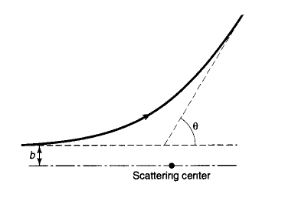
\includegraphics[scale=1.2]{ClassicalScattering}
\end{center}
\newpage

\subsection{Solving for differential cross-section}
Particles incident within an infinitesimal patch of cross-sectional area d$\sigma$ will scatter into a corresponding infinitesimal solid angle dQ. 
The larger d$\sigma$ is, the bigger dQ will be; the proportionality factor, D($\theta$) = d$\sigma$/dQ, is called the differential (scattering) cross-section, and is given by,

\begin{equation}
	d\sigma=D(\theta)d\Omega
\end{equation}
In terms of the impact parameter and the azimuthal angle $\phi, d\sigma = b.db.d\phi$ and $d\Omega=\sin(\theta)d\theta d\phi$, and so,

\begin{equation}
	D(\theta)=\frac{b}{\sin\theta}\abs{\frac{db}{d\theta}}
\end{equation}
And then the total cross-section is the integral of D($\theta$) over all solid angles,

\begin{equation}
	\sigma=\int D(\theta)d\Omega
\end{equation}

The differential cross-section is the total area of incident beam that is scattered by the target. Beams incident within this area will hit the target, and those farther out will miss it completely.\\
If we have a beam of incident particles, with uniform intensity/luminosity ($\mathcal{L}$), the number of particles entering area d$\sigma$ (and hence scattering into solid angle d$\Omega$), per unit time, is dN = $\mathcal{L}$d$\sigma$= $\mathcal{L}$D($\theta$)d$\Omega$, then,

\begin{equation}
	D(\theta)=\frac{1}{\mathcal{L}}\frac{dN}{d\Omega}
\end{equation}

This is the definition of the differential cross-section.

\begin{center}
	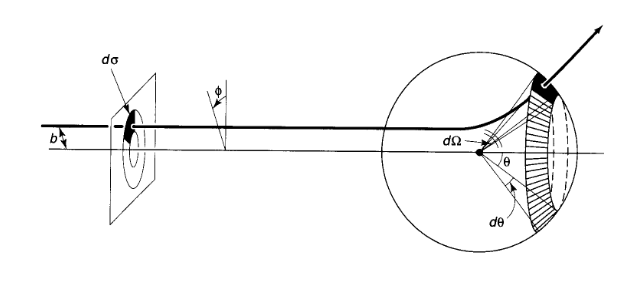
\includegraphics[scale=0.8]{DiffScattering}
\end{center}
\newpage


\section{Quantum Scattering}
\subsection{Defining the problem}
In the quantum theory of scattering, we imagine an incident plane wave,$\psi(z)=Ae^{ikz}$ , traveling in the z
direction, which encounters a scattering potential, producing an outgoing spherical wave That is, we look for solutions to the Schrödinger equation of the generic form,

\begin{equation}
	\psi(r,\theta)\approx A\left\{e^{ikz}+f(\theta)\frac{e^{ikr}}{r}\right\} \textrm{,	for large $r$}
\end{equation}

The relation between wave number $k$ and energy of incident particles are,
\begin{equation}
	k\equiv \frac{\sqrt{2mE}}{\hbar}
\end{equation}
\subsection{Determining scattering amplitude}
Probability of the incident particle travelling with speed $v$ passing through infinitesimal area $d\sigma$ in time $dt$ is,
\begin{equation}
	dP=\vert \psi_{incident}\vert^2dV=\vert A \vert^2(v dt)d\sigma
\end{equation}
This is equal to the probability that the particle later emerges into the corresponding solid angle $d\Omega$,
\begin{equation}
	dP=\vert \psi_{scattered}\vert^2dV=\frac{\vert A \vert^2\vert f \vert^2}{r^2}(v dt)r^2d\sigma
\end{equation}
And $d\sigma$=$\vert f\vert^2d\Omega$, so,
\begin{equation}
	D(\theta)=\frac{d\sigma}{d\Omega}=\vert f(\theta)\vert^2
\end{equation}
The differential cross-section (which is the quantity of interest to the experimentalist) is equal to the	absolute square of the scattering amplitude. Now we look at different methods to determine this scattering amplitude.

\newpage

\section{Partial Wave Analysis}
\subsection{Formalism}
We know that the Schrodinger equation for a spherically symmetrical potential $V(r)$ admits the separable solutions,
\begin{equation}
	\psi(r,\theta,\phi)=R(r)^m_l(\theta,\phi)
\end{equation}
Where $Y^m_l$ is a spherical harmonic and $u(R)=rR(r)$ satisfies the radial equation,
\begin{equation}
	-\frac{\hbar^2}{2m}\frac{dl^2 u}{d r^2} + \left[V(r) + \frac{\hbar^2}{2m}\frac{l(l+1)}{r^2}\right]u = Eu
\end{equation}
At very large $r$, the potential goes to zero, and the centrifugal term is negligible, so,
\begin{equation}
	\frac{d^2u}{dr^2}\approx-k^2u
\end{equation}
Whose general solution is takes the form,
\begin{equation}
	u(r)=Ce^{ikr}+De^{-ikr}
\end{equation}
The first term represents an outgoing spherical wave, and the second an incoming one. For the scattered wave, we want $D=0$. At very large r, then.
\begin{equation}
	R(r)\approx\frac{e^{ikr}}{r}
\end{equation}
The radial equation then becomes,
\begin{equation}
	\frac{d^2}{dr^2}-\frac{l(l+1)}{r^2}u=-k^2u
\end{equation}
The general solution for the radial equation is a linear combinations of spherical Bessel functions,
\begin{equation}
	u(r)=Arj_l(kr)+Brn_l(kr)
\end{equation}		
We need solutions that are linear combinations analogous to $e^ikr$ and $e^-ikr$, these are called the spherical Hankel functions,
\begin{equation}
	h^{(1)}_l\equiv j_l(x)+in_l(x)
\end{equation}
\newpage
Below we see some examples of Hankel functions,

\begin{center}
	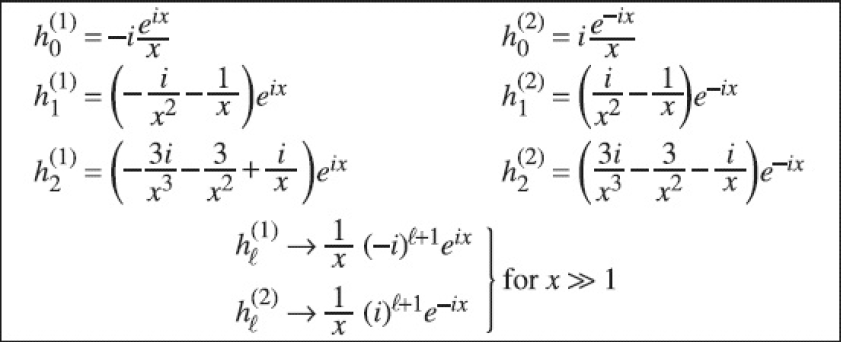
\includegraphics[scale=0.8]{Hankels}
\end{center}
The Hankel function of the first kind becomes $e^-ikr/r$ for large r, so we use these to get,
\begin{equation}
	R(r)=Cj^{(1)}_l(kr)
\end{equation}
\subsection{Exact wavefunction and the partial wave amplitude}
The exact wave function in the exterior region where $V(r)=0$ is,
\begin{equation}
	\psi(r,\theta,\phi)=A\left\{e^{ikz}+f(\theta,\phi)\frac{e^{ikr}}{r}\right\}
\end{equation}
Where,
\begin{equation}
	f(\theta,\phi)+\frac{1}{k}\sum_{l,m}^{}(-i)^{l+1}C_{l,m}Y^m_l(\theta,\phi)
\end{equation}
The $C_{l,m}$ are called the partial wave amplitudes. Now the cross section is,
\begin{equation}
	D(\theta,\phi)= \vert f(\theta,\phi)\vert^2= \frac{1}{k^2} \sum_{l,m}\sum_{l',m'}(i)^{l-l'}C^*_{l,m}C_{l'm'}(Y^m_l)^*Y^{m'}_{l'}
\end{equation}
And the total cross-section is,
\begin{equation}
	\sigma= \frac{1}{k^2} \sum_{l,m}\sum_{l',m'}(i)^{l-l'}C^*_{l,m}C_{l'm'}\int(Y^m_l)^*Y^{m'}_{l'}d\Omega=\frac{1}{k^2}\sum_{l,m}^{}\vert C_{l,m}\vert ^2
\end{equation}
We know from the Legendre functions that,
\begin{equation}
	Y^0_l(\theta,\phi)=\sqrt{\frac{2l+1}{4\pi}}P_l(cos\theta)
\end{equation}
where $P_l$ is the $l$th Legendre Polynomial. Now the exact wave function in the exterior region is,
\begin{equation}
	\psi(r,\theta)=A\left\{e^{ikz}+\sum_{l=0}^{\infty}\sqrt{\frac{2l+1}{4\pi}}C_lh_l^{(1)}(kr)P_l(cos\theta)\right\}
\end{equation}
The scattering amplitude is now given by,
\begin{equation}
	f(\theta)=\frac{1}{k}\sum_{l=0}^{\infty}(-i)^{l+1}\sqrt{\frac{2l+1}{4\pi}}C_lP_l(cos\theta)
\end{equation}
and the total cross-section is,

\begin{equation}
	\sigma=\frac{1}{k^2}\sum_{l=0}^{\infty}|C_l|^2
\end{equation}
To fix the hybrid notation of the cartesian incoming wave and the spherical outgoing wave, we write it in a more consistent form.\\ 
We know that the general solution to the Schrodinger equation with $V=0$ can be written in the form,
\begin{equation}
	\sum_{l,m}^{}[A_{l,m}j_l(kr)+B_{l,m}n_l(kr)]Y^m_l(\theta,\phi)
\end{equation}
Expanding the plane wave in terms of spherical waves using Rayleigh's formula,
\begin{equation}
	e^{ikz}=\sum_{l=0}^{\infty}i^l(2l+l)j_l(kr)P_l(cos\theta)
\end{equation}
Substituting this in Equation (24), the consistent exterior region wave function can be written as,
\begin{equation}
	\psi(r,\theta)=A\left[l(2l+l)j_l(kr)+\sum_{l=0}^{\infty}\sqrt{\frac{2l+1}{4\pi}}C_lh_l^{(1)}(kr)\right]P_l(cos\theta)
\end{equation}

\section{Phase Shift}
Let's begin by considering a one-dimensional scattering problem with a localized potential on the half-line $x < 0$ and a brick wall at $x = 0$. So a wave incident from the left,
\begin{equation}
\psi_{i}(x) = A e^{ikx}
\end{equation}
is entirely reflected,
\begin{equation}
\psi_{r}(x) = B e^{-ikx}
\end{equation}
\begin{figure}[h]
	\centering
	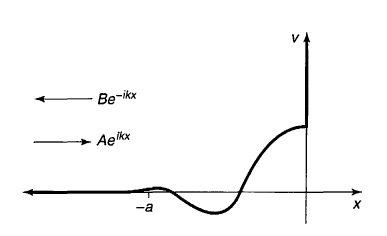
\includegraphics[scale=0.6]{1d_scatt.png}
	\caption{1D scatterubg frin a localized potential bounded on the right by an infinite wall}
\end{figure}
where $x < -a$. No matter what happens in $-a < x < 0$ (the interaction region), the amplitude (amplitude in the context of waves not probability amplitude) of the reflected wave is the same as the incident wave simply due to conservation of probability. However, the two waves need not have the same phase. If there were no potential at all ($V(x) = 0$), but just at the wall ($x = 0$), then $B = -A$, since the total wave function, incident + reflected must vanish at the origin,
\begin{equation}
\psi_{0} = A (e^{ikx} - e^{-ikx})
\end{equation}
If the potential is not zero ($V(x) \neq 0$), then the wave function ($x < -a$) takes the form:
\begin{equation}
\psi = A \left(e^{ikx} - e^{i(2 \delta - kx)} \right)
\end{equation}
Thus, the whole scattering problem reduces to the problem of calculating the phase shift $\delta$ as a function of $k$ and hence of the Energy $E = \hbar^{2}k^{2}/2m$. Yes there's a factor of 2, before $\delta$, but that's only conventional. We think of the incident wave as being phase shifted once on the way in and again on the way out. Thus, by $\delta$ we mean the one-way phase shift and $2\delta$ the total phase shift. We go about this by solving the Schrodinger equation in $-a < x < 0$ along with relevant boundary conditions. Why are we working with $\delta$ rather than the complex amplitude $B$? It makes the physics and math simpler:
\begin{itemize}
\item \textbf{Physically:} We only need to think of the conservation of probability. The potential merely shifts the phase
\item \textbf{Mathematically:} We trade a complex number for a real one
\end{itemize}
Let's return to the 3D  case. The incident plane wave carries no angular momentum in the z direction. Thus Rayleigh's formula contains no terms with $m \neq 0$ but insteaed it cfontains all values of the total angular momentum ($l = 0, 1, 2$). Since angular momentum is conserved by a spherically symmetric potential each partial wave labelled by a particular $l$ scatters independently with no change in amplitude (amplitude in this context refer to the amplitude of the wave no the probability amplitude) but differing in phase. If there is no potential then $\psi_{0} = A e^{ikx}$ and the $l$th partial wave is
\begin{equation}
\psi^{l}_{0} = A i^{l} (2l +1) j_{l}(kr)P_{l}(\cos(\theta))
\end{equation}
But from our previous considerations,
\begin{equation}
j_{l}(x) = \frac{1}{2} \left[h^{(1)}(x) + h^{2}_{l}(x) \right] \approx \frac{1}{2x} \left[(-i)^{l+1} e^{ix} + i^{l+1}e^{-ix} \right]
\end{equation}
for $x >>1$. So for large $r$,
\begin{equation}
\psi^{(l)}_{0} \approx A \frac{2l + 1}{2ikr} \left[e^{ikr} - {(-1)}^{l}e^{-ikr}\right] P_{l}(\cos(\theta))
\end{equation}
The second term in square brackets corresponds to an incoming spherical wave. It is unchanged when we introduce the scattering potential. The first term is the outgoing wave. It picks up a phase shift $\delta_{l}$:
\begin{equation}
	\label{tobeass}
\psi^{(l)} \approx A \frac{2l + 1}{2ikr} \left[e^{i(kr + 2\delta_{l})} - {(-1)}^{l}e^{-ikr}\right] P_{l}(\cos(\theta))
\end{equation}
Think of it as a converging spherical wave due to the $h^{(2)}_{l}$ component in $e^{ikz}$, which is phase shifted by $2\delta_{l}$ and emerges as an outgoing spherical wave i.e. the $h^{l}_{l}$ part of $e^{ikz}$ as well  as the scattered wave itself. In the previous section the whole theoryu was expressed in terms of partial wave amplitudes $a_{l}$, now we have formulated it in terms of the phase shifts $\delta_{l}$. There must be a connectioni between the two. Well if we take the assymptotic i.e. large $r$ limit of eq. (\ref{tobeass}):
\begin{equation}
\psi^{(l)} \approx A\left( \frac{(2l + 1)}{2ikr} \left[e^{i(kr + 2\delta_{l})} - {(-1)}^{l}e^{-ikr}\right] + \frac{(2l + 1)}{r}a_{l}e^{ikr} \right) P_{l}(\cos(\theta))
\end{equation}
With the generic expression in terms of $e^{i \delta_{l}}$ we find
\begin{equation}
a_{} = \frac{1}{2ik}(e^{2i \delta_{l}} - 1) = \frac{1}{k} e^{i \delta_{l}} \sin(\delta_{l})
\end{equation}
Although we used the assymptotic form of the wave function to find the connection there's nothing approximate about the result. Both of them are constants independent of $r$ and $\delta_{l}$ means the phase shift in the asymptotic region i.e. where the Hankel functionis have settled down to $e^{\pm ikr}/kr$. It follows in particular that,
\begin{equation}
f(\theta) = \frac{1}{k}\sum_{l=0}^{\infty}(2l + 1)e^{i \delta_{l}} \sin(\delta_{l}) P_{l}(\cos(\theta)) 
\end{equation}
and,
\begin{equation}
\sigma = \frac{4 \pi}{k^{2}} \sum_{l=0}^{\infty}(2l + 1) \sin[2](\delta_{l})
\end{equation}
Voila!
\section{Born Approximation}
\subsection{Integral Form of the Schrodinger Equation}
Before we even head to deriving the "Integral Form of the Schrodinger Equation". Why you might ask? It will become evident in the upcoming sections. So let's begin by recalling the time-independent Schrodinger equation
\begin{equation}
\frac{num}{2m} + V \psi = E \psi
\end{equation}
We can rewrite this as,
\begin{equation}
(\nabla^{2} + k^{2}) \psi = Q
\end{equation}
where
$$k = \frac{\sqrt{2mE}}{\hbar}$$
$$Q = \frac{2m}{\hbar^{2}}V \psi$$
This looks pretty similar to the Helmholtz equation from electrodynamics. Here however the "inhomogeneous" term Q itself depends on $\psi$
Suppoase we could find a function that solves the Helmholtz equation with a delta function source:
\begin{equation}
	content...
\end{equation}
We can then express as an integral:
\begin{equation}
	\psi() = \int
\end{equation}
$G(\vec{r})$ is called the Green's function for the Helmholtz equation. Moreover, generally speaking the Green's function for a linear differential equation represents the response to a delta function.
Note that $G + G_{0}$ still satisfies Equation (). This is simply due to the multivalued nature of the holomorphic function. Thus, the integral form of the Schrodinger equation can be written as,
\begin{tcolorbox}
\begin{equation}
\psi(\vec{r}) = \psi_{0}(\vec{r}) - \frac{m}{2 \pi \hbar^{2}}\int\frac{e^{ik\abs{\vec{r} - \vec{r}_{0}}}}{\abs{\vec{r} - \vec{r}_{0}}}  V(\vec{r}_{0}) \psi(\vec{r}_{0}) d^{3}\vec{r}_{0}
\end{equation}
\end{tcolorbox}
Let's see how this helps us.
\subsection{The First Born Approximation}
Suppose $V(\vec{r}_{0})$ is localized about r = 0, that is the potential drops to 0 after a finite region and we want to calculate $\psi(\vec{r})$ at points distant from the scattering center. Then for all points that contribute to the integral form of the Schrodinger equation. So,
\begin{equation}
\abs{\vec{r} - \vec{r}_{0}} = r^{2} + r_{0}^{2} - 2\vec{r}\vec{r_{0}}  \approxeq r^{2} \left(1 - 2\frac{\vec{r}.\vec{r}_{0}}{r^{2}} \right)
\end{equation}
and hence,
\begin{equation}
\abs{\vec{r} - \vec{r}_{0}} \approxeq r - \hat{r} . \vec{r}_{0}
\end{equation}
Let,
\begin{equation}
\vec{K} = k \hat{z}
\end{equation}
then
\begin{equation}
e^{-i \vec{K}\abs{\vec{r} - \vec{r}_{0}}} \approx e^{ikr}e^{-i \vec{K}.\vec{r}_{0}}
\end{equation}
and therefore,
\begin{equation}
\frac{e^{-i \vec{K}\abs{\vec{r} - \vec{r}_{0}}}}{\abs{\vec{r} - \vec{r}_{0}}} \approx \frac{e^{ikr}}{r}e^{-i \vec{K}.\vec{r}_{0}}
\end{equation}
In the case of scattering, we want:
\begin{equation}
\psi_{o}(\vec{r}) = Ae^{ikz}
\end{equation} 
to represent an incident plane wave. For large $r$,
\begin{equation}
\psi \approxeq Ae^{ikz} - \frac{m}{2 \pi \hbar^{2}A} \int e^{-i \vec{K}.\vec{r}_{0}}V(\vec{r}_{0})\psi(\vec{r}_{0})d^{3}\vec{r}_{0}
\end{equation}
This is in the standard form. We can read off the scattering amplitude:
\begin{equation}
f(\theta, \phi) = \frac{m}{2 \pi \hbar^{2}A} \int e^{-i \vec{K}.\vec{r}_{0}}V(\vec{r}_{0})\psi(\vec{r}_{0})d^{3}\vec{r}_{0}
\end{equation}
So far this is exact. Now we invoke the Born approximation: "Suppose the incoming plane wave is not substantially altered by the potential; then we can say that
\begin{equation}
\psi(\vec{r}_{0}) \approxeq \psi_{0}(\vec{r}_{0}) = A e^{ikz_{o}} = A e^{i\vec{K}^{'}\vec{r}_{o}}
\end{equation}
where
$$K^{'}= k \hat{z}$$
inside the integral. This would be just the wave function if $V$ were zero. It is essentially just a weak potential approximation. Generally partial wave analysis is useful when the incident particle has low energy the only the first few terms in the series contribute significantly. The Born approximation applies when the potential is weak when compared to the incident energy, thus the deflection is small. In the Born approximation then,
\begin{tcolorbox}
	\begin{equation}
		f(\theta, \phi) \approxeq -\frac{m}{2 \pi \hbar^{2}} \int e^{i(k^{'}-k). \vec{r}_{0}}V({r}_{0})d^{3}\vec{r}_{0}
	\end{equation}
\end{tcolorbox}
In particular, for low energy scattering, the exponential factor is essentially constant over the scattering region and the Born approximation simplifies to:
\begin{tcolorbox}
	\begin{equation}
		f(\theta, \phi) \approxeq -\frac{m}{2 \pi \hbar^{2}} \int V(\vec{r}) d^{3}r
	\end{equation}
\end{tcolorbox}
For a spherically symmetrical potential, $V(\vec{r}) = V(r)$ but not necessarily at low energy. The Born approximation reduces to a simpler form. First we define:
\begin{equation}
\mathcal{K} = k^{'} - k
\end{equation}
and let the polar axis for the $r_{0}$, the integral lies along so that;
\begin{equation}
(k^{'} - k).r_{0} = \mathcal{K}r_{0} \cos(\theta_{0})
\end{equation}
Then,
\begin{equation}
f(\theta) \approxeq -\frac{m}{2 \pi \hbar^{2}} \int e^{i \mathcal{K} r_{0} \cos(\theta_{0})} V(\theta_{0}) r^{2}_{0} \sin(\theta_{0}) dr_{0}d \theta_{0} d \phi_{0}
\end{equation}
The integral is trivial, $2\pi$, and the integral $\theta_{0}$ is on we have encountered before in equation (). Dropping the subscript on $r$, we are left with
\begin{tcolorbox}
\begin{equation}
f(\theta) \approxeq -\frac{2m}{\hbar^{2} \mathcal{K}} \int_{0}^{\infty} rV(r)\sin(\mathcal{K}r) dr
\end{equation}
\end{tcolorbox}
The angular dependence of $f$ is carried by $\mathcal{K}$. From our previous considerations we can see that:
\begin{equation}
\mathcal{K} = 2k \sin(\theta /2)
\end{equation}
\subsection{Examples}
\subsubsection{Low-energy soft-sphere scattering}
Note: We can't apply the Born approximationi to hard-sphere scattering as the integral blows up due to our assumption (i.e. potential does not affect the wave function) here. Suppose,
\begin{equation}
	V(\vec{r}) = \begin{cases}
		V_{0}, & \text{ if } r \leq a \\
		0, & \text{ if } r > a
	\end{cases}
\end{equation}
In this case the low-energy scattering amplitude is,
\begin{equation}
	f(\theta, \phi) \approxeq -\frac{m}{2 \pi \hbar^{2}}V_{0}\left(\frac{4}{3} \pi a^{3} \right)
\end{equation}
This is independent of $\theta$ and $\phi$ ! Thus, the differential cross-section is:
\begin{equation}
\frac{d \sigma}{d \Omega} = \abs{f}^{2}  \approxeq \left[\frac{2m V_{0} a^{3}}{3 \hbar^{2}} \right]^{2}
\end{equation}
and the total cross-section:
\begin{equation}
\sigma 	\approxeq 4 \pi \left(\frac{2m V_{0} a^{3}}{3 \hbar^{2}}\right)^{2}
\end{equation}
\subsubsection{Yukawa Scattering}
The Yukawa potential is a toy-model for the binding force in the nucleus of an atom. It has the form,
\begin{equation}
V(r) = \beta \frac{e^{-\mu r}}{r}
\end{equation}
where $\beta$ and $\mu$ are constants. The Born approximation gives,
\begin{equation}
f(\theta) \approxeq -\frac{2m \beta}{\hbar^{2}k} \int_{0}^{\infty} e^{- \mu r} \sin(kr) dr = - \frac{2m \beta}{\hbar^{2} (\mu^{2} + k^{2})}
\end{equation}
\subsubsection{Rutherford Scattering}
If we substitute $\beta = q_{1}q_{2}/ 4 \pi \epsilon_{0}$ and $\mu = 0$. The scattering amplitude is given by,
\begin{equation}
f(\theta) \approxeq - \frac{2m q_{1}q_{2}}{4 \pi \epsilon_{0} \hbar^{2} k^{2}}
\end{equation}
or,
\begin{equation}
f(\theta) \approxeq - \frac{q_{1}q_{2}}{16 \pi \epsilon_{0} E \sin[2](\theta / 2)}
\end{equation}
The differential cross-section is the square of this:
\begin{equation}
	\frac{d \sigma}{d \Omega} = \left[\frac{q_{1}q_{2}}{16 \pi \epsilon_{0} E \sin[2](\theta / 2)} \right]^{2}
\end{equation}
\subsection{The Born series}
The Born approximation is very similar to the impulse approximation in the contex of classical scattering. 
\begin{figure}[h]
	\centering
	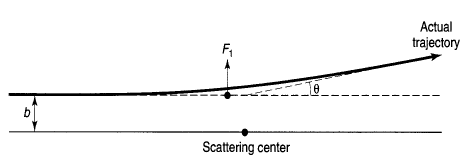
\includegraphics[scale=0.5]{impulse_scatt.png}
	\caption{An example of the impulse approximation: the particle continues undeflected}
\end{figure}
In that sector we start by assuming that the particle keeps going in a straight line and compute the transverse impulse that would be delivered to it in that case:
\begin{equation}
I = \int F_{\perp} dt
\end{equation}
If the deflection is small in comparism to the motion, it would then be a good approximation to the transverse momentum supplied to th particle. Thus we express the scattering angle as:
\begin{equation}
\theta = \arctan(I/p)
\end{equation}
where $p$ is th incident momentum. This is the "first-order" impulse approximation. The zeroth-order is what we started wtih i.e. no deflection at all. Likewise, in the zeroth-order Born approximation the incident plane wave passes by with no modification and what we saw earlier was just the first order correction to this. But the same pattern of thought can lead us to a series which then leads us to higher-order corrections. Let's recall the integral form of the Schrodinger equation:
\begin{equation}
		\label{schrod_int_2}
	\psi (\vec{r}) = \psi_{0} (\vec{r}) + \int g(\vec{r} - \vec{r}_{0})V(\vec{r}_{0})\psi(\vec{r}_{0})d^{3}r_{0}
\end{equation}
where is the incident wave and,
$$g(\vec{r}) = -\frac{m}{2 \pi \hbar^{2}}\frac{e^{ikr}}{r}$$
is the Green's function with a factor $m/2 \pi \hbar^{2}$ for convenience and $V$ is the scattering potential.
Suppose we take the equation for $\psi$ and plug it back into (\ref{schrod_int_2}),
$$\psi = \psi_{0} + \int g V\psi_{0} + \int \int g V g V\psi$$
Iterating this we obtain the series expasion for $\psi$,
\begin{equation} 
	\label{dysonseries}
\psi = \psi_{0} + \int g V\psi_{0} + \int \int g V g V\psi_{0} + \int \int \int g V g V g V\psi_{0} ...
\end{equation}
\begin{figure}[h]
	\label{born_diag}
	\centering
	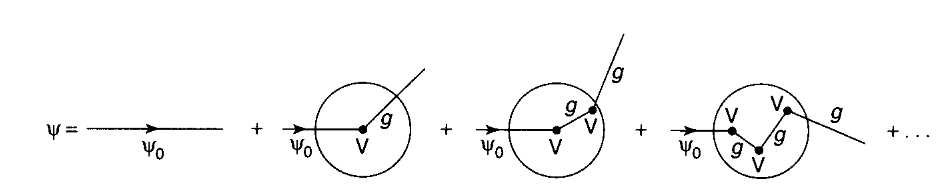
\includegraphics[scale=0.5]{born_series.png}
	\caption{A diagram representing the Born series}
\end{figure}
We notice the following from (\ref{dysonseries}):
\begin{itemize}
\item The first Born approximation truncates the series after the Next to Leading Order (NLO) term
\item In the Leading Order $\psi$ is untouched by $V$
\item In the first order (Next to Leading Order) it is kicked once
\item In the second order it is kicked, propagates to a new location and is kicked again and so on
\item In this context the Green's function is essentially just the propagator \footnote{In this context it tells us how the disturbance propagates between one interaction and the next}
\item This was in fact the inspiration for Feynman diagrams which is expressed in terms of vertex factors ($V$) and propagators ($g$)
\end{itemize}
Figure (\ref{born_diag}) might look familiar, because it closely represents Feynman diagrams.
\begin{figure}[h]
	\centering
	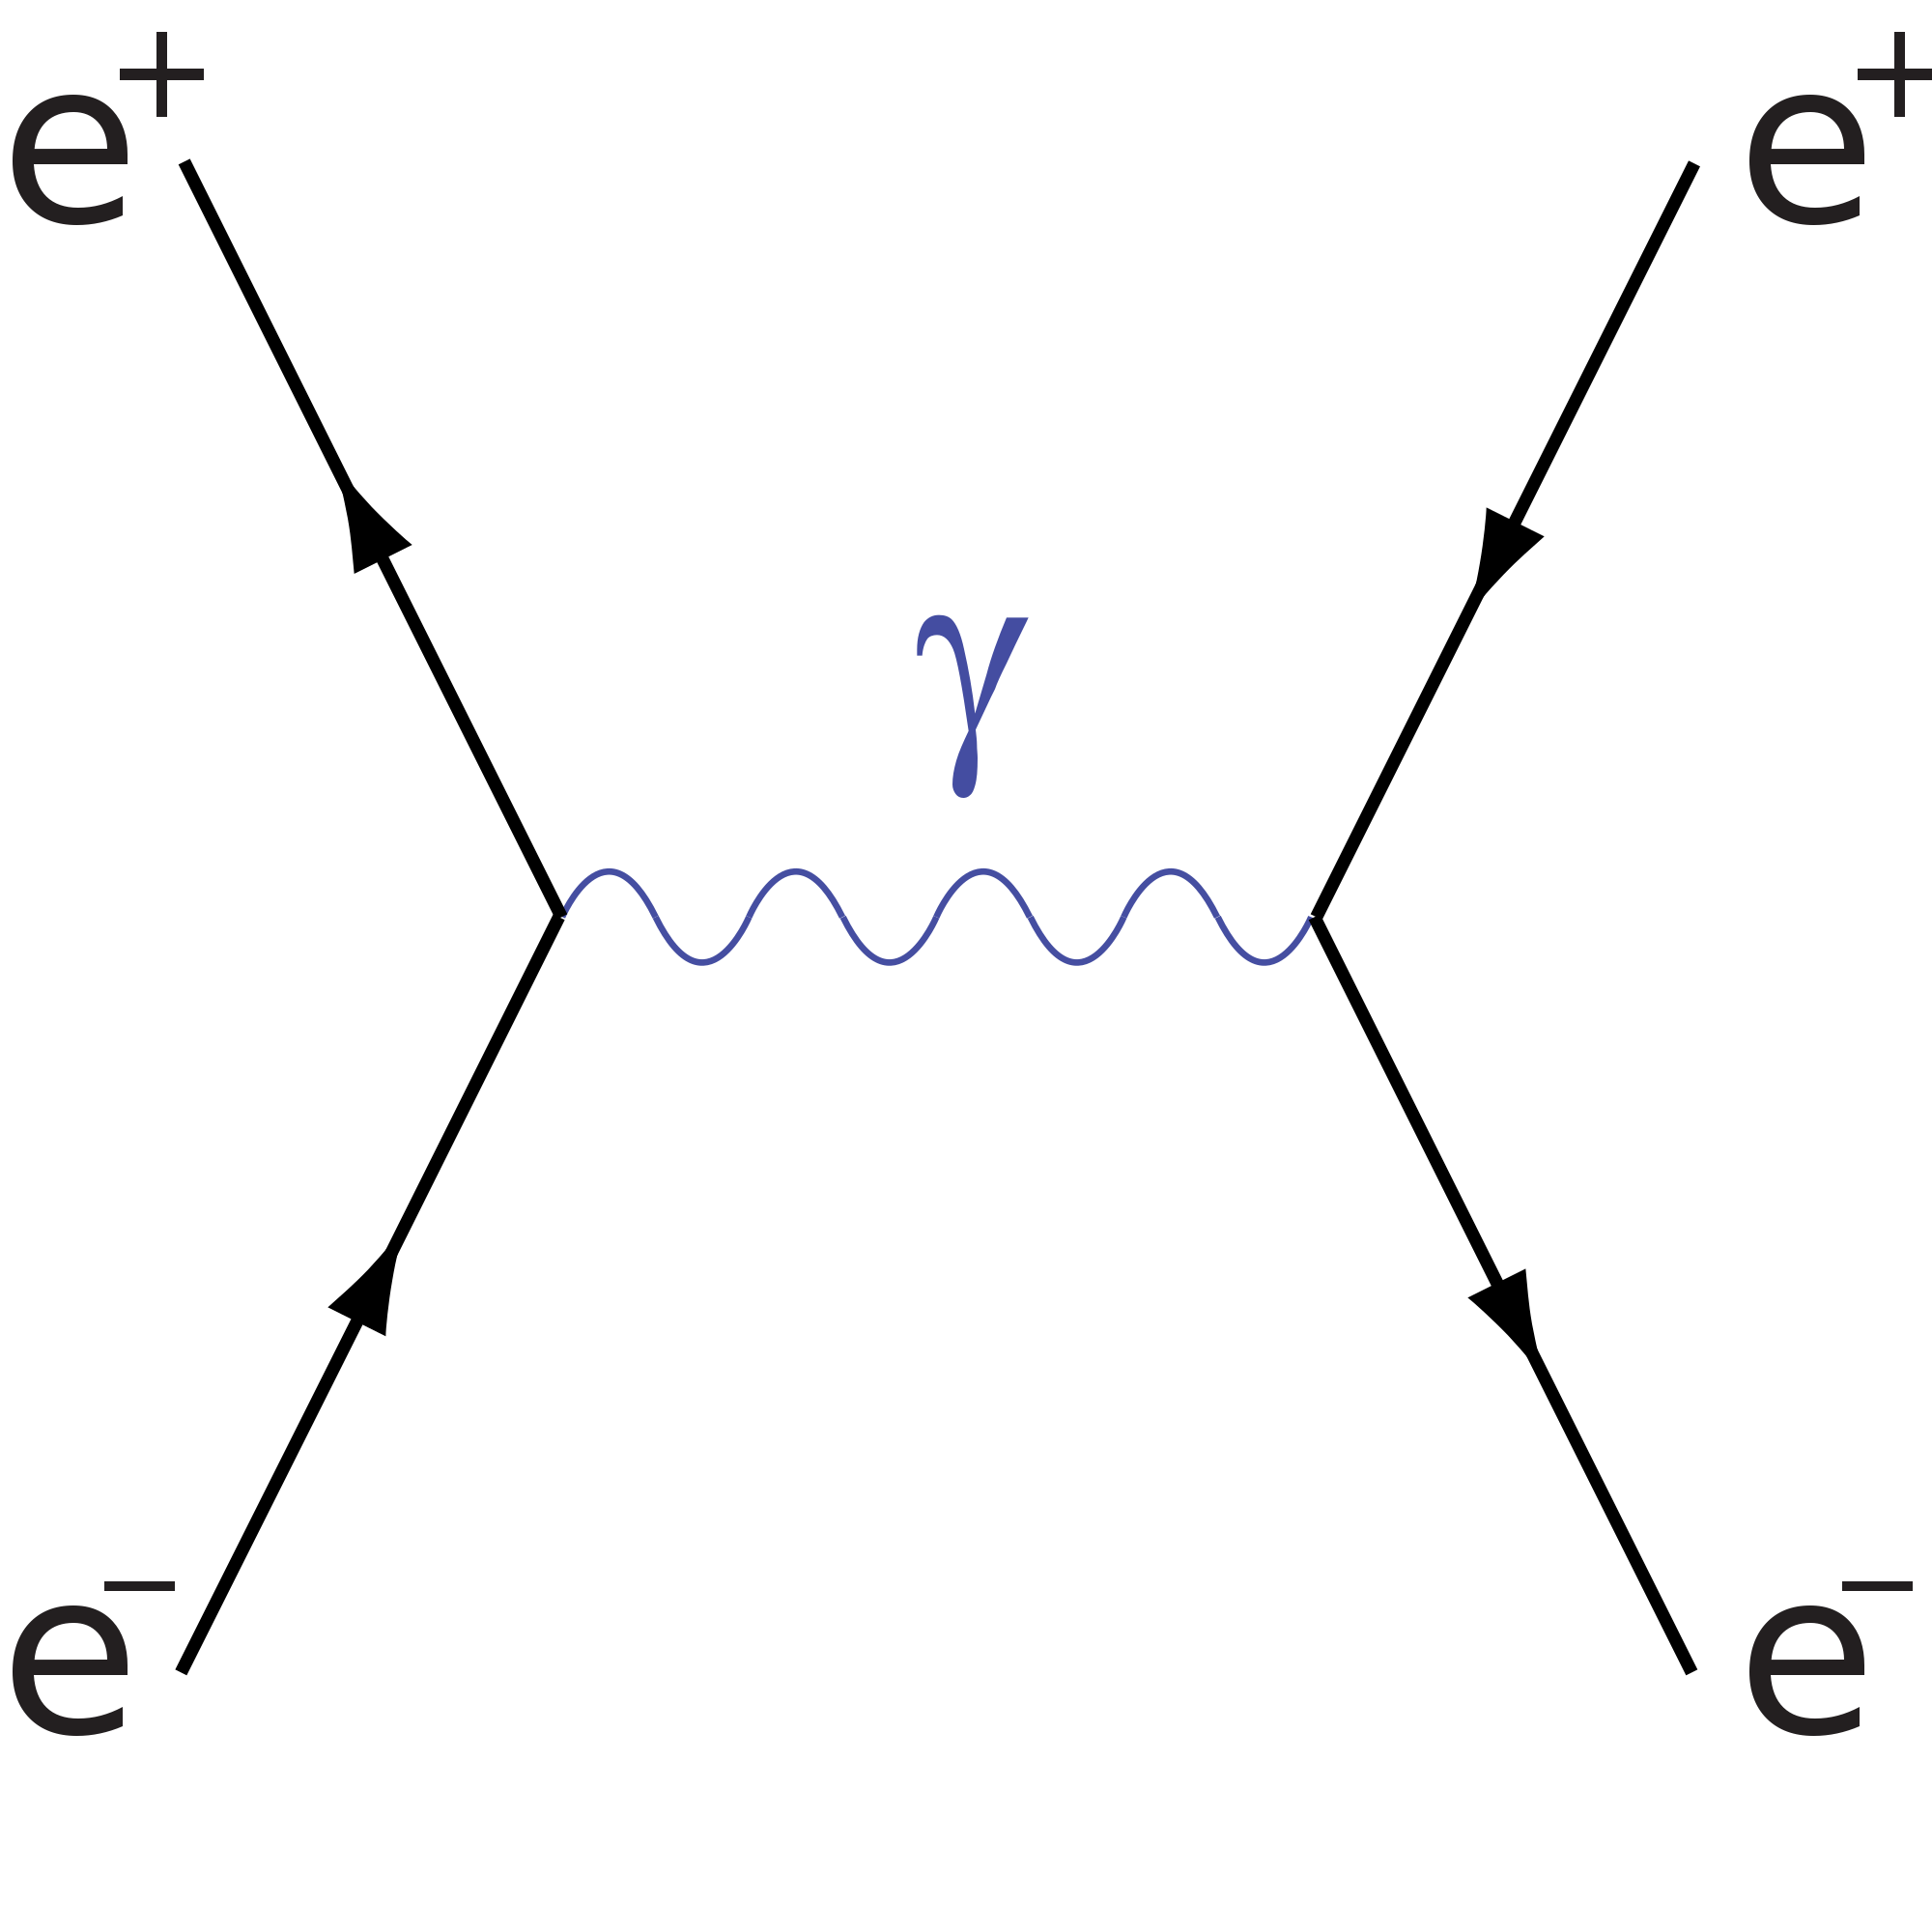
\includegraphics[scale=0.1]{2000px-Bhabha_S_channel.svg}
	\caption{Bhabha scattering: Annihilation}
\end{figure}